\documentclass[9pt]{beamer}

\usetheme[{titleformat plain}=smallcaps,
          titleformat title=smallcaps,
          titleformat subtitle=regular,
          titleformat section=smallcaps,
          titleformat frame=smallcaps,
          numbering=fraction
          ]{metropolis}
\usepackage{appendixnumberbeamer}

\usepackage{booktabs}
\usepackage[scale=2]{ccicons}

\usepackage{tikz}
\usetikzlibrary{shapes,arrows}
\usepackage{amsmath, bm}
\usepackage{physics,hepnames}
\usepackage{mathtools}

\usepackage{subfig}

\usepackage{pgfplots}
\usepgfplotslibrary{dateplot}

\usepackage{xspace}
\usepackage{soul}
\newcommand{\themename}{\textbf{\textsc{metropolis}}\xspace}

\DeclareMathOperator{\msbar}{\overline{MS}}
\DeclareMathOperator{\dis}{DIS}
\DeclareMathOperator{\phys}{PHYS}
\DeclareMathOperator{\pos}{POS}
\DeclareMathOperator{\dpos}{DPOS}
\DeclareMathOperator{\mpos}{MPOS}

\title{Can $\msbar$ PDF be negative?}
%\subtitle{arXiv:2006.07377}
\date{February, 2020}
\author{Alessandro Candido
}
%\institute{N3PDF}
\titlegraphic{
%        \raisebox{5pt}[0pt][0pt]{
\includegraphics[height=0.8cm]{../_logos/nnpdf_logo.pdf}}\hspace*{10pt}
        \hfill
        \raisebox{5pt}[0pt][0pt]{
\includegraphics[height=0.8cm]{../_logos/n3pdf_logo.pdf}}\hspace*{10pt}
        
\includegraphics[height=1.3cm]{../_logos/erc_logo1.png}

        \vfill\vspace*{170pt}
        
\includegraphics[height=1cm]{../_logos/unimi_logo.png}\hfill
        
\includegraphics[height=1cm]{../_logos/infn_logo.png}\\
        \vspace*{5pt}
        {\fontsize{3pt}{3.5pt}\selectfont
             \begin{center}
                 This project has received funding from the European Union's Horizon 2020 research and innovation programme under grant agreement No 740006\quad 
\includegraphics[height=5pt]{../_logos/eu-flag.jpg}
         \end{center}}
}

\begin{document}

\maketitle

\begin{frame}{Table of contents}
  \setbeamertemplate{section in toc}[sections numbered]
    \tableofcontents%[hideallsubsections]
\end{frame}

\section{Parton model}
\begin{frame}{Introduction}
    \begin{columns}
        \begin{column}{0.7\textwidth}
            The \textit{parton model} consist in a model of the proton
            structure as a bunch of free components, collectively called
            \textit{partons}:

            \begin{itemize}
                \item in principle any elementary particle
                \item in practice mostly \textbf{quarks} and \textbf{gluons}
            \end{itemize}

            \vspace*{15pt}
            It has been historically formulated as a model before the theory of
            quarks, just assuming \textbf{point-like constituents} for the
            proton, now it has a special role as a model because some of its
            properties\footnotemark can be deduced from field theory and
            Standard Model.
        \end{column}
        \begin{column}{0.3\textwidth}
            \begin{figure}
                \centering
                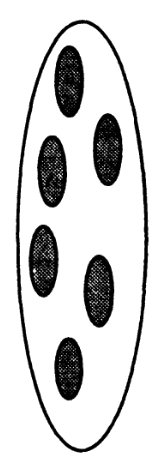
\includegraphics[height=150pt]{pictures/partons}
            \end{figure}
        \end{column}
    \end{columns}

    \footnotetext{The actual structure of the proton has a non-perturbative
    origin, so it cannot be completely understood by perturbative QFT}
\end{frame}


\begin{frame}{LO PDF definition}
    \begin{columns}
        \begin{column}{0.55\textwidth}
            Since they are free the main property of each parton is the
            fraction of the total momentum it carries.\newline

            The probability distribution of finding a parton $p$ with momentum
            fraction $x$ it's encoded in its \textit{Parton Density Function}\footnotemark,
            $f_p(x)$.
        \end{column}
        \begin{column}{0.45\textwidth}
            Plot LO PDFs

            %\begin{figure}
                %\centering
                %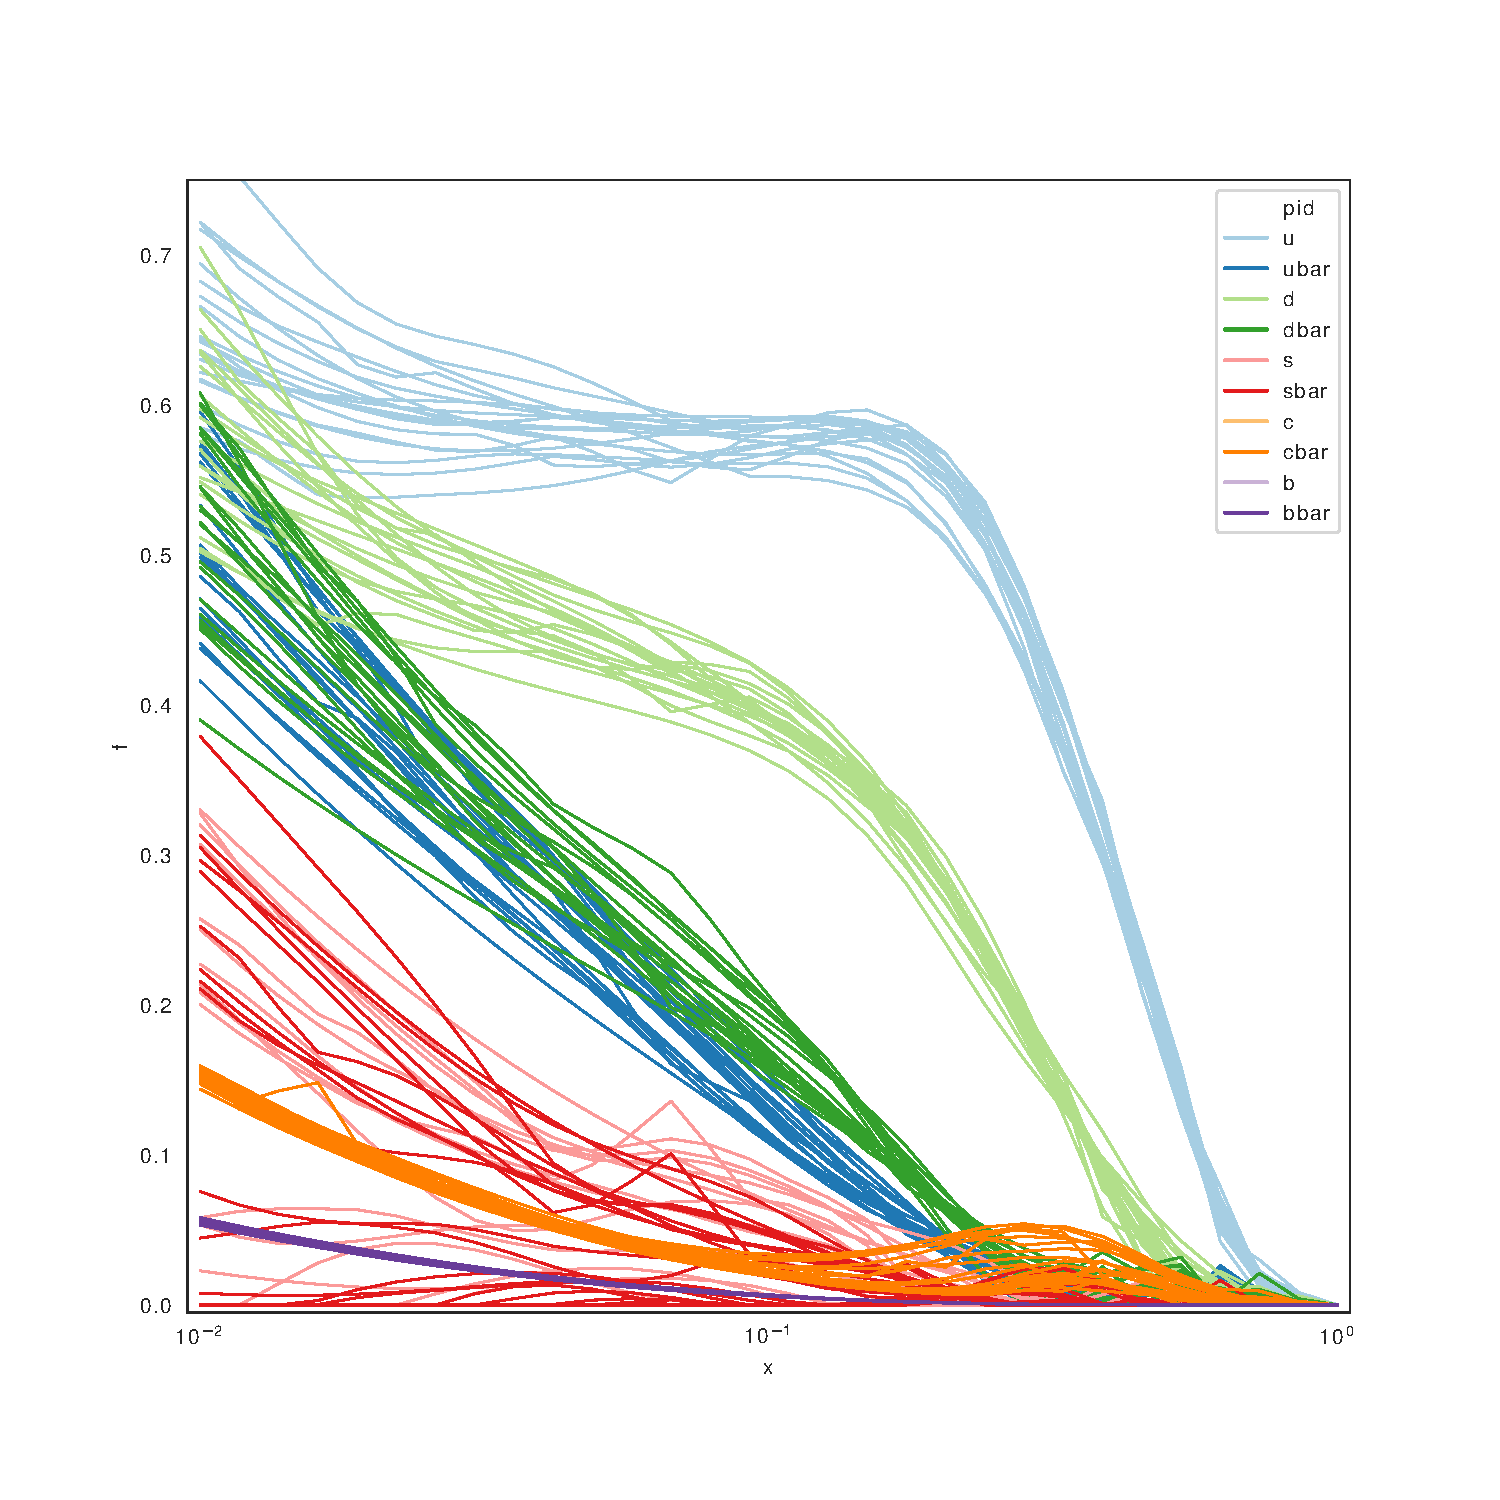
\includegraphics[height=150pt]{pictures/lo_pdfs}
            %\end{figure}
        \end{column}
    \end{columns}
    \footnotetext{In general PDFs also depend on the energy scale $Q^2$, but at
    LO they scale (see \textit{Björken scaling}). This statement can be
    explained by perturbative QCD and systematically improve, including the
    dependency through $\alpha_s$.}
\end{frame}

\section{PDF @ NLO: factorization scheme}
\begin{frame}{NLO divergences}
    As well known at NLO divergences start to appear, both in virtual and real contributions.
    \begin{figure}
        \centering
        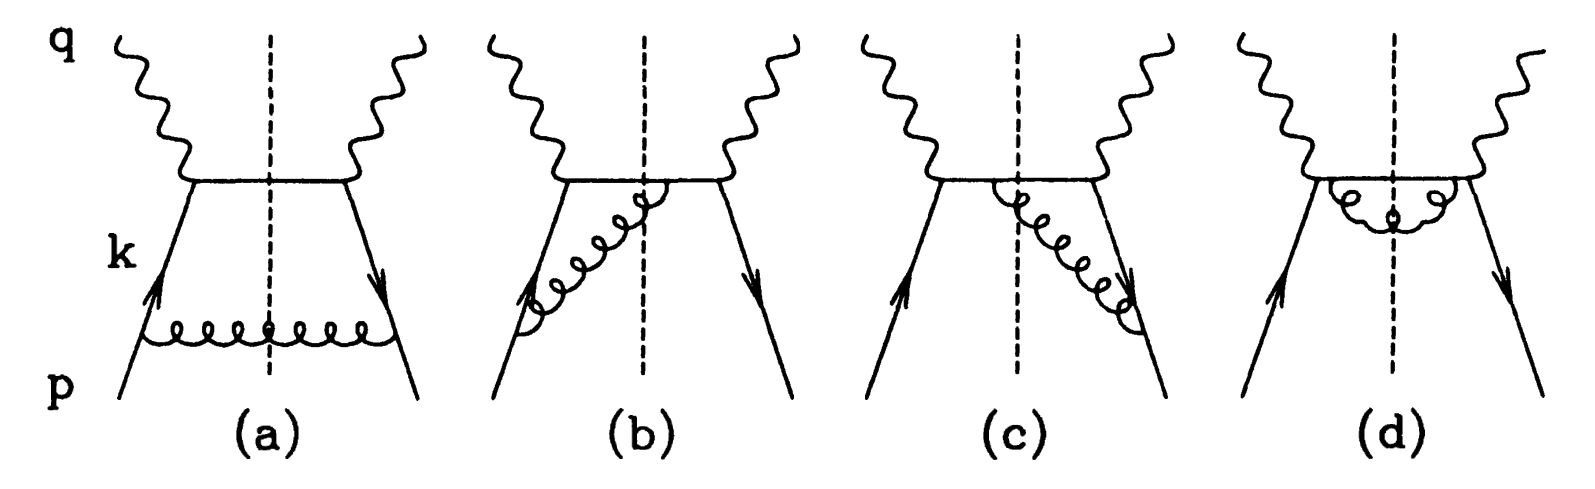
\includegraphics[width=.8\textwidth]{pictures/nlo-real}
    \end{figure}
    There are 3 kinds of divergences:
    \begin{itemize}
        \item \textbf{virtual}, due to loop integrals
        \item \textbf{soft}, due to emission of an extra soft particle
        \item \textbf{collinear}, due to
    \end{itemize}
    The first two kinds are known to cancel in sufficiently inclusive
    observables\footnote{e.g.: the KLN theorem is one of the results that guarantee
    this cancellation.}.
\end{frame}

\begin{frame}{NLO collinear divergences}
    On the other hand collinear divergences have \textit{a different origin}
    that can be related to the asymptotic freedom of strong interactions:

    \begin{center}
        \textit{The collinear limit corresponds to a long range (soft) part of
        the strong interaction, which is not calculable in perturbation
        theory.}
    \end{center}

    These divergences must be treated in a different way, defining a suitable
    \textbf{factorization scheme}.\newline

    Notice that collinear divergences are also responsible for the appearance
    of the characteristic $\alpha_s \log(Q^2)$, that will introduce the PDF
    dependency on $Q^2$.
\end{frame}

\begin{frame}{Factorization Scheme}
    \vspace*{15pt}
    The way to deal with these divergences is offered by the previous
    interpretation: we can hide them in a non-perturbative object, the PDF.
    \begin{align*}
        F_2(x,Q^2) &= x\sum_{q,\bar{q}} q_0 \otimes \hat{F}_{2,0} (x, Q^2) =
        x \sum_{q,\bar{q}} \int\limits_x^1 \frac{\dd\xi}{\xi} q_0(\xi)
        \hat{F}_{2,0}\left(\frac{x}{\xi},Q^2\right)\\
        &= x \sum_{q,\bar{q}} q \otimes \hat{F}_2 (x, Q^2)\\
    \end{align*}
    \vspace*{-15pt}

    Example: DIS scheme for DIS @ NLO
    \begin{align*}
        \hat{F}_{2,0}(x,Q^2) &= e_q^2 x \left[ \delta(1-x) +
        \frac{\alpha_s}{2\pi}\left(P(x) \log(\frac{Q^2}{\kappa^2}) +
        C(x)\right) + \dots \right]\\
        q(x, \mu^2_F) &= q_0(x) + \frac{\alpha_s}{2\pi} \int\limits_x^1
        \frac{\dd \xi}{\xi} q_0(\xi) \left\{ P\left(\frac{x}{\xi}\right)
        \log(\frac{\mu^2_F}{\kappa^2}) + C\left(\frac{x}{\xi}\right)\right\} +
        \dots
    \end{align*}
\end{frame}

\begin{frame}{Factorization Scheme}
    This will result:
    \begin{itemize}
        \item in the effective \textit{subtraction} of the collinear divergence
            in the partonic cross section
        \item the definition of a "renormalized" PDF
        \item the appearance of a new unphysical energy scale: $\mu_F$, the
            \textit{factorization scale} (which is on the same ground of $\mu_R$).
    \end{itemize}

    There is an \textbf{arbitrariness} on defining the finite part of the
    subtraction, in the very same way of the renormalization scheme.

    However, since the subtraction is related to a redefinition of the PDFs,
    once that a scheme has been \textbf{chosen} (fixing a finite subtraction)
    it should be kept for all the processes, because the \textbf{PDFs are
    always the same}.
\end{frame}

\begin{frame}{Factorization Scheme (CS counterterm)}
    The formula for a cross section in a generic factorization scheme can be
    written as an additional counterterm contribution $\dd\sigma^C_a$, in this
    case coming from the PDF redefinition:
    \begin{align*}
        \sigma_a^{NLO}(p; \mu_F^2) &= \int\limits_{m+1} \dd\sigma^R_a(p) +
        \int\limits_{m} \dd\sigma^V_a(p) + \int\limits_{m} \dd\sigma^C_a(p;
        \mu_F^2)\\
        \dd\sigma^C_a(p;\mu_F^2) &= - \frac{\alpha_s}{2\pi}
        \frac{1}{\Gamma(1-\epsilon)} \sum_b \int\limits_0^1 \dd z \left[ -
        \frac{1}{\epsilon} \left(\frac{4\pi\mu^2}{\mu_F^2}\right)^\epsilon
        P^{ab}(z) + K^{ab}(z) \right] \dd \sigma_b^B(zp)
    \end{align*}
    in dimensional regularization\footnote{The counterterm is such that
    $K^{ab}=0$ for $\msbar$ factorization scheme}.

    This will be useful in what follows, because it is exactly by choosing a
    specific factorization scheme (i.e. a specific $K^{ab}$ matrix) that we can
    analyze the property of the frequent $\msbar$ choice.
\end{frame}

\section{An intrinsic positive scheme}
\begin{frame}{Is there a positive scheme?}
    At LO PDFs are positive by construction, since they are defined as
    probability distributions, but this is \textbf{not true at NLO}, since we
    \textbf{redefined the PDF} with the \textit{subtraction from the
    factorization scheme}.\newline

    So the question:

    \begin{center}
        \textit{Does it exist at all a factorization scheme in which PDF are\\ still positive also @ NLO?}
    \end{center}

    And the answer can be ready given: \textbf{Yes}.\newline

    It results that there is not a single positive scheme, and there is a
    particularly simple class of them.
\end{frame}

\begin{frame}{A physical scheme}
    A special class of factorization scheme is the one in which the PDFs are
    directly defined on \textbf{physical observables}, subtracting \textit{all
    of the finite} contribution.

    Like in the DIS scheme we can choose two physical processes for defining the quark and gluon PDF:
    \begin{description}
        \item[quark] we can choose a hypothetical $\bar{q} p \to \gamma^* + X$
        (Drell-Yan with a pure antiquark beam), or a DIS structure function;
        \item[gluon] either a hypothetical $g p \to H + X$ (gluon fusion with a
        pure gluon beam), or a photon-gluon fusion;
    \end{description}
\end{frame}

\begin{frame}{The $\phys$ scheme}
    We can choose one of these schemes and call it $\phys$, for example:
    \begin{align*}
        \frac{1}{x}\bar{\sigma}(x,Q^2) &= f^{\,\phys}(x,Q^2)\\
        \bar{\sigma}(x,Q^2) &= \begin{pmatrix}
        \sigma(x,Q^2)[\bar{q} p \to \gamma^* + X]\\
        \sigma(x,Q^2)[g p \to H + X]
        \end{pmatrix}
    \end{align*}

    As one can deduce from the first equation this scheme is positive by
    construction, since the PDF is proportional to a physical cross-section,
    whose positivity is guaranteed.
\end{frame}

\section{Coefficient functions NLO behaviour}
\begin{frame}{Universality of collinear structure}
    In $\msbar$ the subtracted cross section can be negative: negative finite
    parts are factored away from the regularized cross sections, into the PDFs,
    that can become negative as well.

    On the other hand, the residue of the collinear pole is universal—it is
    given by process-independent splitting functions $P_{ab}$.
    %If all contributions which are factored away from the partonic cross
    %section and into the PDF remain positive, then the latter also stays
    %positive.
    \begin{figure}
        \begin{tabular}{cc}
          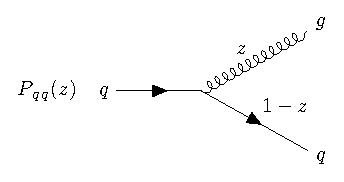
\includegraphics[width=0.3\textwidth]{pictures/feynd/Pqq} &   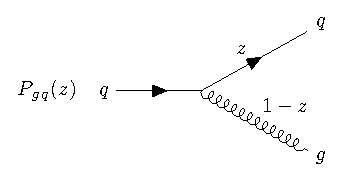
\includegraphics[width=0.3\textwidth]{pictures/feynd/Pgq} \\
          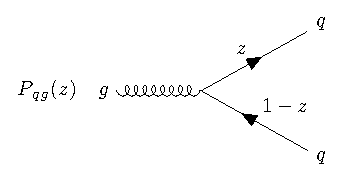
\includegraphics[width=0.3\textwidth]{pictures/feynd/Pqg} &   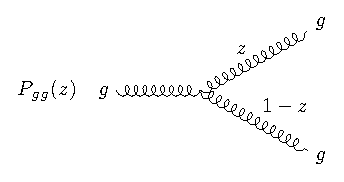
\includegraphics[width=0.3\textwidth]{pictures/feynd/Pgg} \\
        \end{tabular}
    %\caption{caption}
    \end{figure}

    For this reason we can go on with the analysis of some particular process
    to catch the universal behavior involved in the factorization scheme.
\end{frame}

\begin{frame}{DIS coefficient functions}
    The DIS structure function, written in terms of the PDFs and the coefficient functions is:
    \begin{equation*}
        \frac{1}{x} F_2(x,Q^2)= e_q^2 \left[q
        +\frac{\alpha_s}{2\pi}\left( C^{(1)}_q \otimes q+ C^{(1)}_g \otimes
        g\right)\right](Q^2)\,,
    \end{equation*}

    \vspace*{15pt}
    \begin{block}{Gluon coefficient}
        The following is the $d$-dimensional, unsubtracted, gluon coefficient function:
        \begin{equation*}
            \label{eq:cgeps}
            C^{(1)}_{g}(x,Q^2,\epsilon) = \frac{ \Gamma(-\epsilon)
            \left(\frac{\mu_D^2}{\pi\mu^2}\right)^{-\epsilon} \left[8P_{qg}(x)-16 T_R \epsilon (3
            -\epsilon(2 -\epsilon) )  \right]  }{16\pi (2 - 2\epsilon) \Gamma (3 - 2 \epsilon)}\,,
        \end{equation*}
        where
        \begin{equation*}
            \label{eq:mud}
            \mu_D^2\equiv|k_T^{\text{max,\,DIS}}|^2=\frac{s}{4}=\frac{Q^2(1-x)}{4x},
        \end{equation*}
    \end{block}
\end{frame}

\begin{frame}{DIS: gluon channel}
    The original $d$-dimensional expression is positive by construction, since
    it is a \textbf{cross-section}, but the $\msbar$ prescription leads to an
    over-subtraction in the gluon channel.

    \begin{figure}
      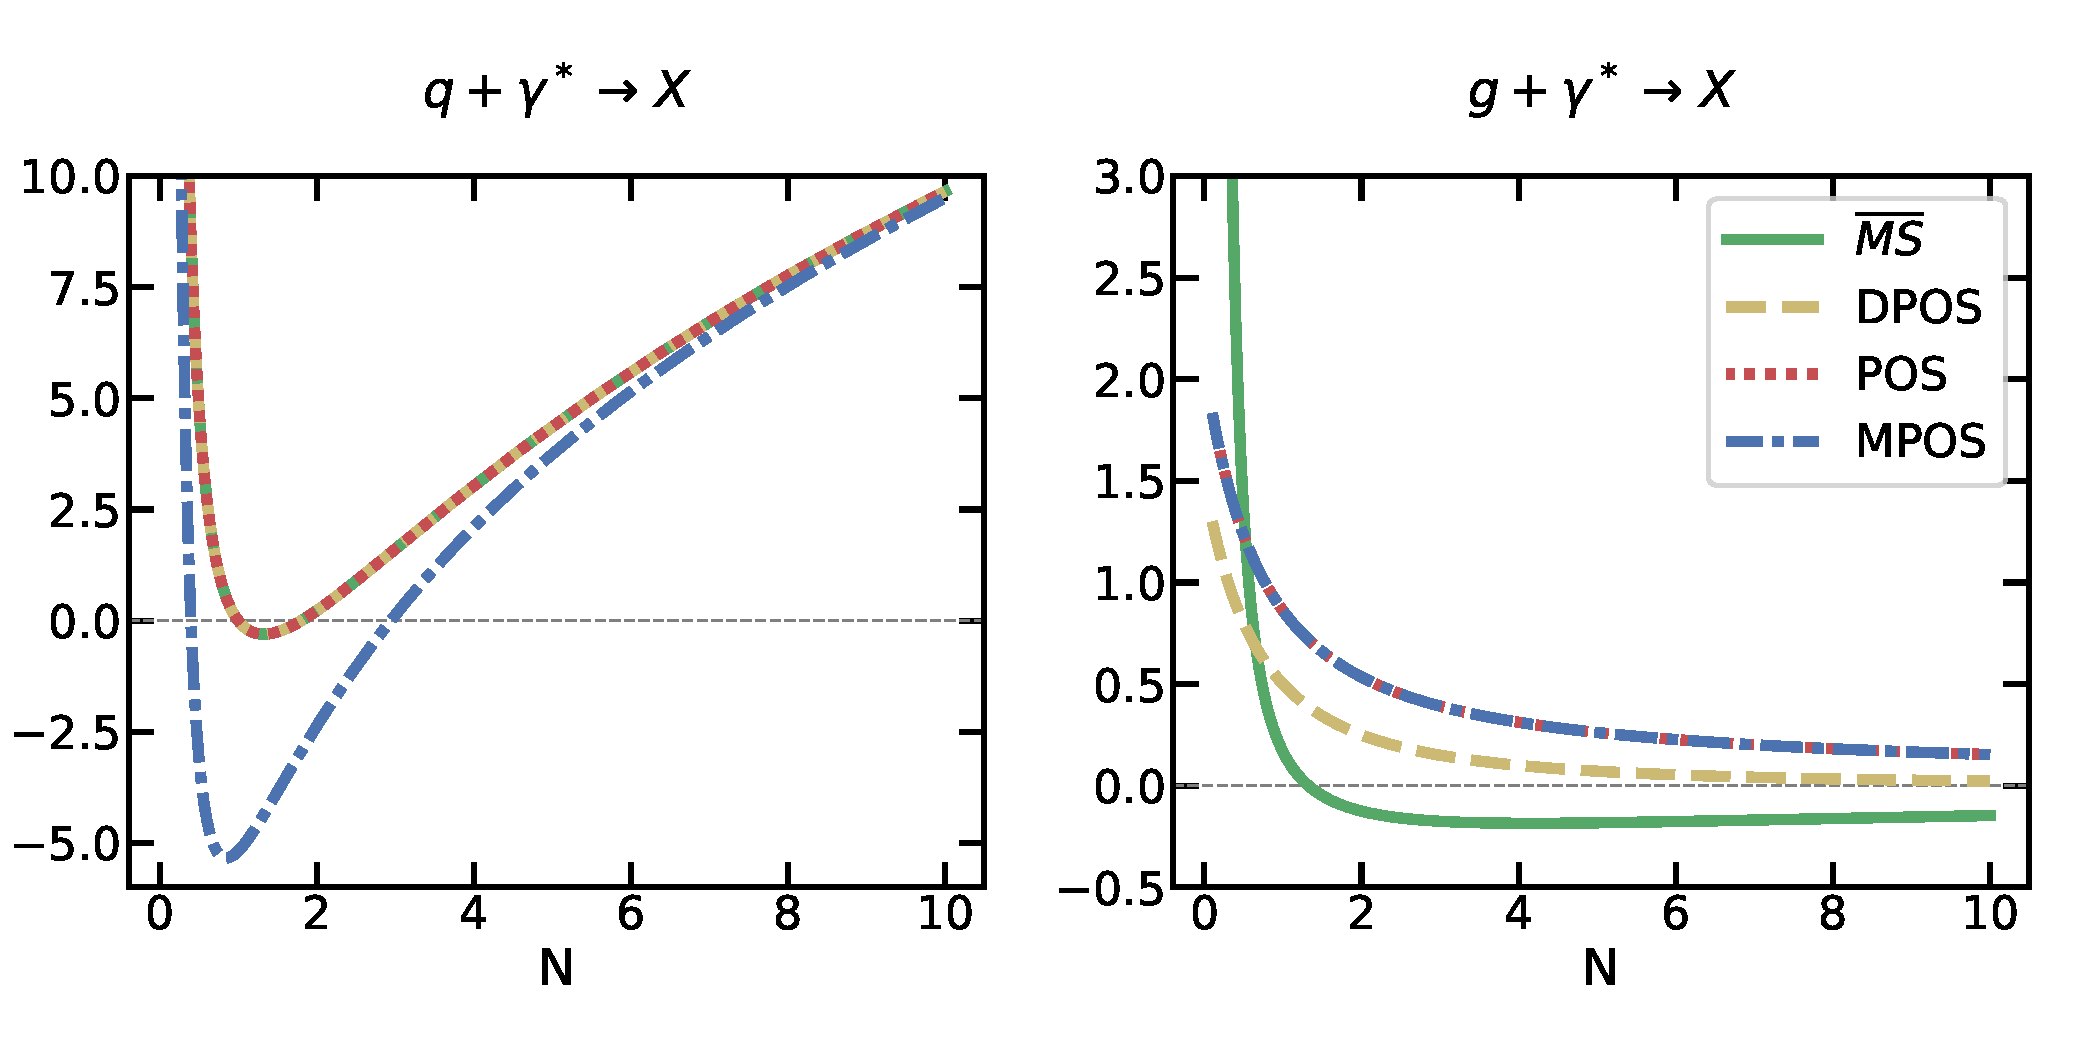
\includegraphics[width=0.85\textwidth]{pictures/dis}
    \end{figure}
\end{frame}

\begin{frame}{DIS: gluon channel}
    We can make it positive again analyzing the source of over-subtraction.

    \begin{align*}\label{eq:cgren}
        {C^{(1)}_{g}}^{\msbar}(x) &= \lim_{\epsilon\to
        0^-}\left[C_{g}^{(1)}(x,Q^2,\epsilon) - \left(\frac{Q^2}{4\pi
        \mu^2}\right)^{-\epsilon} \left(-\frac 1
        {\epsilon}+\gamma_E\right) P_{qg}(x)\right]\\
        {C^{(1)}_{g}}^{\dpos}(x) &= \lim_{\epsilon\to0^-}
        \left[{C^{(1)}_{g}}(x,Q^2,\epsilon) -
        \frac{1}{\alert{1-\epsilon}}\left(\frac{\alert{\mu_D^2}}{\pi\mu^2}\right)^{-\epsilon}
        \left(-\frac 1 {\epsilon}+\gamma_E\right) P_{qg}(x)\right]\\
        &= 3\left[ T_R- P_{qg}(x)\right]
    \end{align*}
    The changes applied have an intrinsic physical meaning:
    \begin{itemize}
        \item the $\dpos$ scheme is subtracting at correct energy scale (maximal transverse momentum, not virtuality)
        \item d-dimensional gluon polarizations' average is taken into account
    \end{itemize}
\end{frame}

\begin{frame}{DIS: ${\tiny \dpos}$ $K$ matrix}
    Applying the definitions of $\msbar$ and $\dpos$ subtraction it is possible
    to define a \textit{change of scheme} matrix $K$:

    \begin{equation*}\label{eq:renorm}
        {C^{(1)}_{g}}^{\rm i}(x) = \lim_{\epsilon\to0^-} {C^{(1)}_{g}}(x,Q^2,\epsilon)
        -\delta_{qg}^i(x,Q^2,\epsilon)\,;\qquad i=\msbar,\> {\tiny\dpos}
    \end{equation*}
    and so:
    \begin{align*}\label{eq:count}
      &   {C^{(1)}_{g}}^{\dpos}(x) =  {C^{(1)}_{g}}^{\msbar}(x) -
      K_{qg}^{\dpos}(x) \,\\
      &  K_{qg}^{\dpos}(x)=\delta_{qg}^{\msbar}-\delta_{qg}^{\dpos}=  P_{qg}(x)\left[\log(\frac{1-x}{x}) - 1\right]
    \end{align*}

    \begin{block}{Quark channel}
    The same procedure can be applied for the \Pq channel, but it results that
    in this case the mismatch is just an \textit{under-subtraction} (see
    previous plot).

    So for the sake of positivity it is fine to choose $K_{qq}^{\dpos}(x) = 0$.
    \end{block}
\end{frame}

\begin{frame}{Incoming gluon and Hadronic processes}
    \vspace*{8pt}
    There are still two elements of matrix missing $K_{qg}^{\dpos}(x)$ and
    $K_{gg}^{\dpos}(x)$, so we need a process with an incoming gluon at LO.

    \vspace*{8pt}
    Moreover there is another consideration that should be taken into account:
    the factorization scheme is linked to collinear structure, that is
    universal \textit{w.r.t. the hard process}, but is affected by the \textbf{incoming
    kinematics}.

    A process the exhibit both of these features is Higgs production via gluon
    fusion $gg\to h + X$ in HEFT\footnote{Also the Drell-Yan process has been
    analyzed in the paper, to isolate the contribution of the different kinematics.}:

    \begin{figure}
      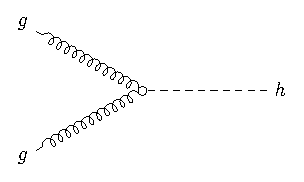
\includegraphics[width=0.45\textwidth]{pictures/feynd/ggh}
    \end{figure}
\end{frame}

\begin{frame}{Hadronic kinematics}
    \vspace*{5pt}
    The equivalent the decomposition of hadronic cross sections in partonic and
    PDFs is:
    \begin{equation*}
        \frac{1}{x} \sigma(x,Q^2)= \hat \sigma_0 \left[  {\cal L}_{ii}
        +\frac{\alpha_s}{2\pi}\left( {{C^i}_q}^{(1)} \otimes {\cal L}_{iq} +
        {{C^i}_g}^{(1)} \otimes {\cal L}_{ig}\right) \right]
    \end{equation*}
    where the parton luminosity is defined as:
    \begin{equation*}\label{eq:lumi}
        {\cal L}_{ij}= f_i\otimes f_j
    \end{equation*}

    \vspace*{10pt}
    As we already stated the only difference is just in the incoming
    kinematics, everything specific to the process is not involved in PDFs
    factorization.

    The quantitative statement is that the only new thing is just the different
    energy available for transverse momentum:
    \begin{equation*}\label{eq:ktmaxh}
        \mu_h^2=  |k_T^{\rm max,\, had}|^2=\frac{(s-Q^2)^2}{4s}=\frac{Q^2(1-x)^2}{4x}
    \end{equation*}
    where $x=\frac{M_H^2}{s}$ and $ Q^2 = M_H^2 $.
\end{frame}


\begin{frame}{Hadronic $K$ matrix}
    It is possible to see that:
    \begin{itemize}
        \item in this case as well there is nothing to be done in the \textbf{diagonal} channel
        \item the \textbf{off-diagonal} matrix element it is similar to the
            DIS, but with a further contribution coming from the second
            incoming particle
    \end{itemize}
    \begin{align*}
        {{C^g{}_g}^{(1)}}^{\pos}(x)  &=  {{C^g{}_g}^{(1)}}^{\msbar}(x)\\
        {{C^g{}_q}^{(1)}}^{\pos} (x) &=  {{C^q{}_g}^{(1)}}^{\msbar} (x) - K_{gq}^{\pos} (x)\\
        K_{gq}^{\pos} (x) &=  P_{gq}(x)\left[\ln\left(\frac{(1-x)^2}{x}\right)
        - 1\right]
    \end{align*}

    And similarly for an incoming quark with the same kind of kinematics, that
    can be deduced from an analogous Drell-Yan process.
\end{frame}

\begin{frame}{Gluon fusion coefficients}
    Since the $\pos$ scheme results to make the DIS cross-sections even more
    positive (non minimal subtraction) it is a good candidate for a positivity
    scheme\footnote{While the one with the DIS kinematics it's not enough to
    make positive hadronic coefficient functions.}.
    \begin{figure}
      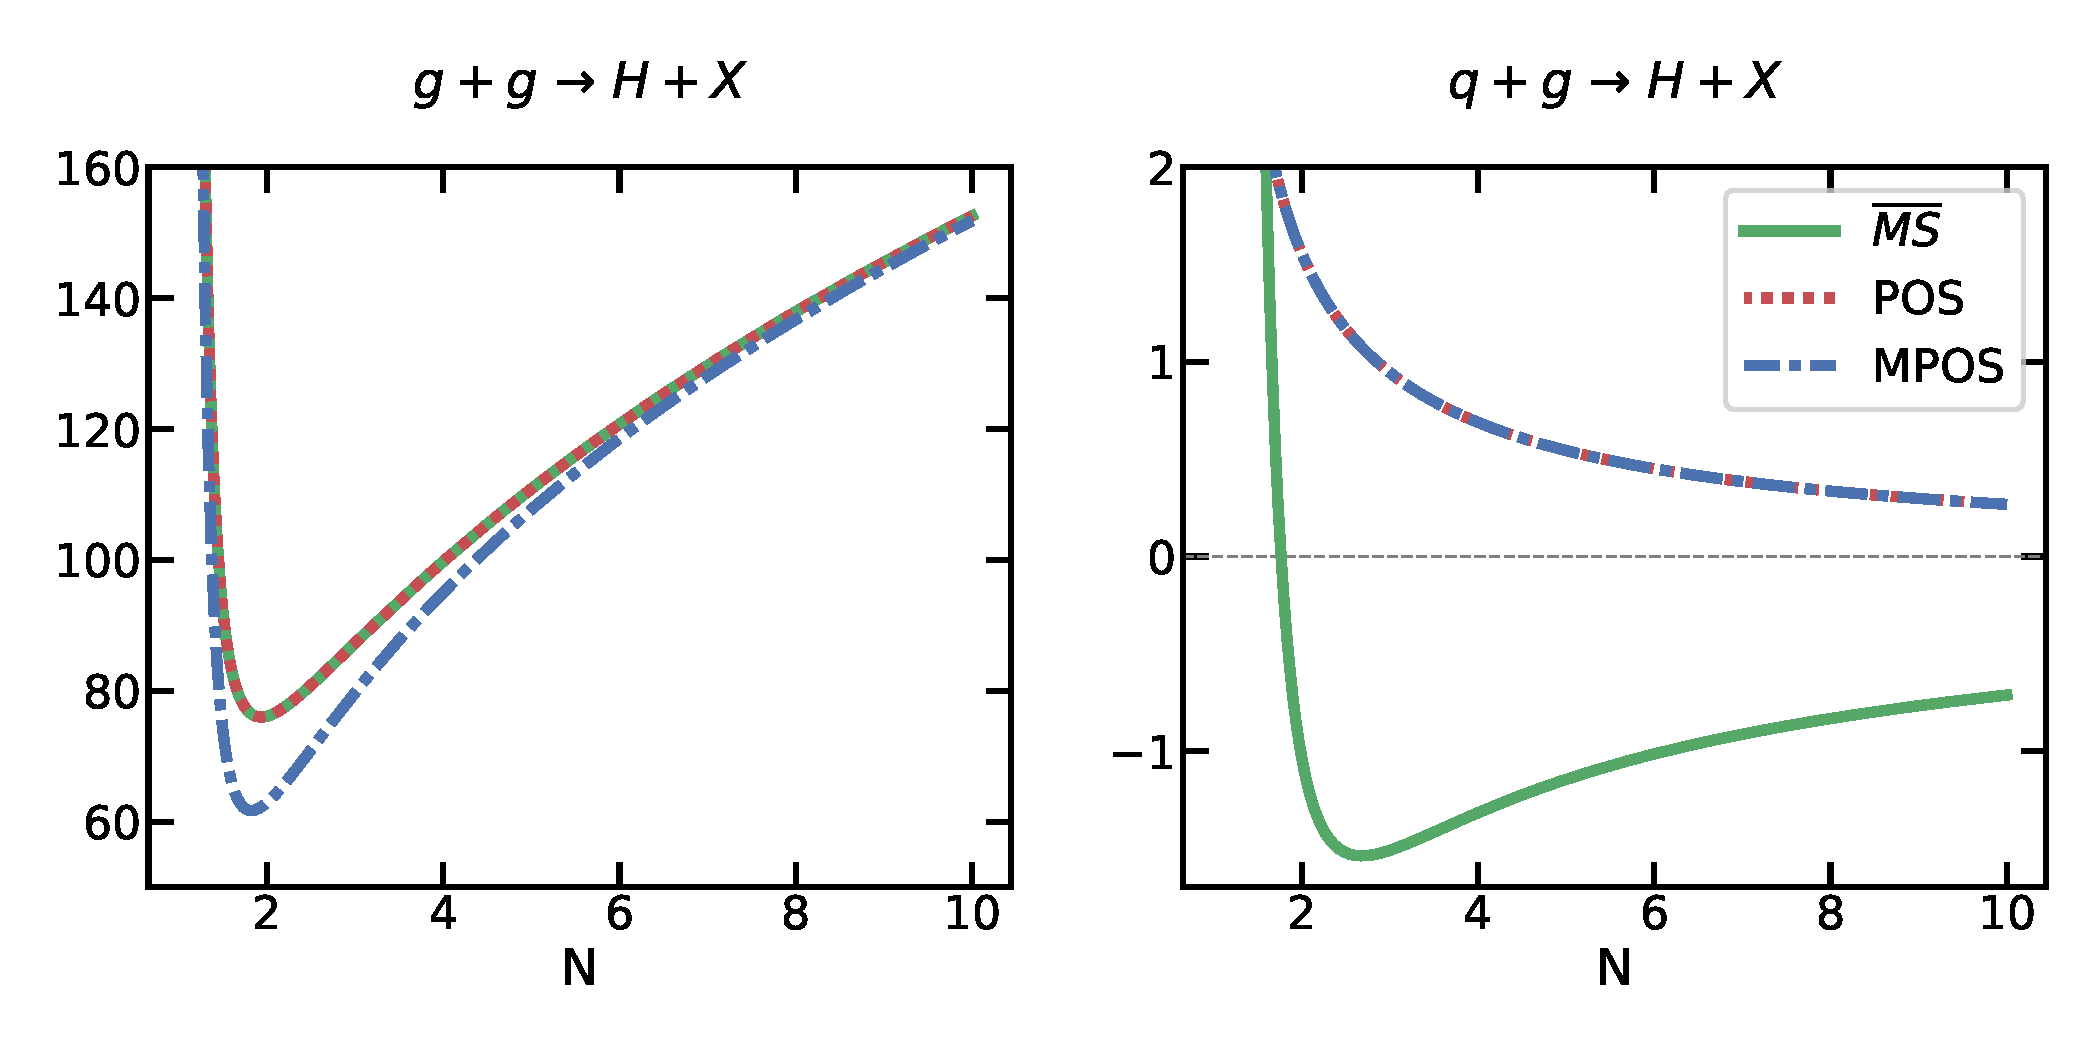
\includegraphics[width=0.85\textwidth]{pictures/higgs}
    \end{figure}
\end{frame}


\section{Is $\msbar$ negative?}
\begin{frame}{Positivity with a single PDF}
    First of all we can consider the case of a \textbf{non-singlet} PDF:
    \begin{equation*}
        q^{\text{NS}}(x, Q^2) = q_i(x, Q^2) - q_j(x, Q^2) \qquad i \neq j
    \end{equation*}
    
    This is \textit{academic} because we are going to \textbf{assume it
    positive in a physical scheme}, but being a \textit{difference} it can also
    not exist such a positive non-singlet.

    \vspace*{15pt}
    Master formula for this part of the argument is:
    \begin{equation*}
        \left[{q^{\text{NS}}}\right]^{\text{DIS}}(x,Q^2)=
        \left[1+\frac{\alpha_s}{2\pi} {\Delta^{(1)}_q}^{\msbar}
        +\frac{\alpha_s}{2\pi}  {\bar
        C^{(1)}_q(x)}^{\msbar}\otimes\right]\left[{q^{\text{NS}}}\right]^{\msbar}(Q^2)
    \end{equation*}
    Coming from the definition of $\left[{q^{\text{NS}}}\right]^{\text{DIS}}$
    as proportional to the physical structure function, and of course of
    $\msbar$ scheme.
\end{frame}

\begin{frame}{Positivity with a single PDF: $\iff C_q(x)^{\msbar} > 0$}
    \begin{block}{Necessity}
        In the equation before the left hand side is known to be positive,
        being physical, but assuming a generic positive $\msbar$ PDF without
        any other restriction means to require the coefficient function to be
        positive.the coefficient function to be positive.the coefficient
        function to be positive.
    \end{block}
    \begin{block}{Sufficiency}
        Applying a \textbf{perturbative inversion} one can find that the
        converse is also true, since the physical (here $\text{DIS}$) PDF is
        positive by construction, and that perturbatively the coefficient
        cannot become negative.

        This is true with a single \textit{caveat}: in the region $1 \to x$ the
        quantity $\alpha_s\log(1-x)$ \textbf{is not small}, so the fixed order
        inversion is not reliable.\\
        One can recover in this case the inverted formula to $\text{LL}(1-x)$,
        showing that the coefficient won't become negative also in this limit.
    \end{block}
\end{frame}

\begin{frame}{The singlet-gluon system}
\end{frame}

\begin{frame}{To a positive $\msbar$}
    Having proved $\mpos$ to be a positive scheme it is rather trivial to show
    the positivity of $\msbar$, because we know the explicit transformation
    between the two schemes:
    \begin{align*}
    \hspace*{-12pt}\left[\mathbb{I}
    +\frac{\alpha_s}{2\pi} {C^{(1)}}^{\msbar}\right]&=\left[\mathbb{I}
      +\frac{\alpha_s}{2\pi} {C^{(1)}}^{\pos}\right]\otimes\left[\mathbb{I}
      +\frac{\alpha_s}{2\pi} {C^{(1)}}^{\pos}\otimes\right]^{-1}\left[\mathbb{I}
      +\frac{\alpha_s}{2\pi}  \left({C^{(1)}}^{\pos} +K^{\pos}\right)\right]\\  
    &=\left[\mathbb{I}
      +\frac{\alpha_s}{2\pi} {C^{(1)}}^{\pos}
      \right]\left[\mathbb{I}
      + \otimes \frac{\alpha_s}{2\pi}  K^{\pos}\right]
    \end{align*}
    and so:
    \begin{equation*}
     f^{\,\pos}(Q^2)=\left[\mathbb{I}
      +\frac{\alpha_s}{2\pi}  K^{\pos}\otimes\right] f^{\,\msbar}(Q^2)\,,
    \end{equation*}
    which inverse can be obtained perturbatively, taking separately into
    account the $x \to 1$ limit in a similar way of what has been done above.
\end{frame}

\begin{frame}{To a positive $\msbar$}
    The explicit expression of the change of scheme matrix $K$ is:
    \begin{equation*}
        K^{\pos}=\left[\ln\left(\frac{(1-x)^2}{x}\right) - 1\right]
        \left(\begin{array}{cc} 0 & P_{qg}(x) \\
        P_{gq}(x) & 0\end{array}\right).
    \end{equation*}
    and its shape in $N$-space can be plotted:
    \begin{figure}
      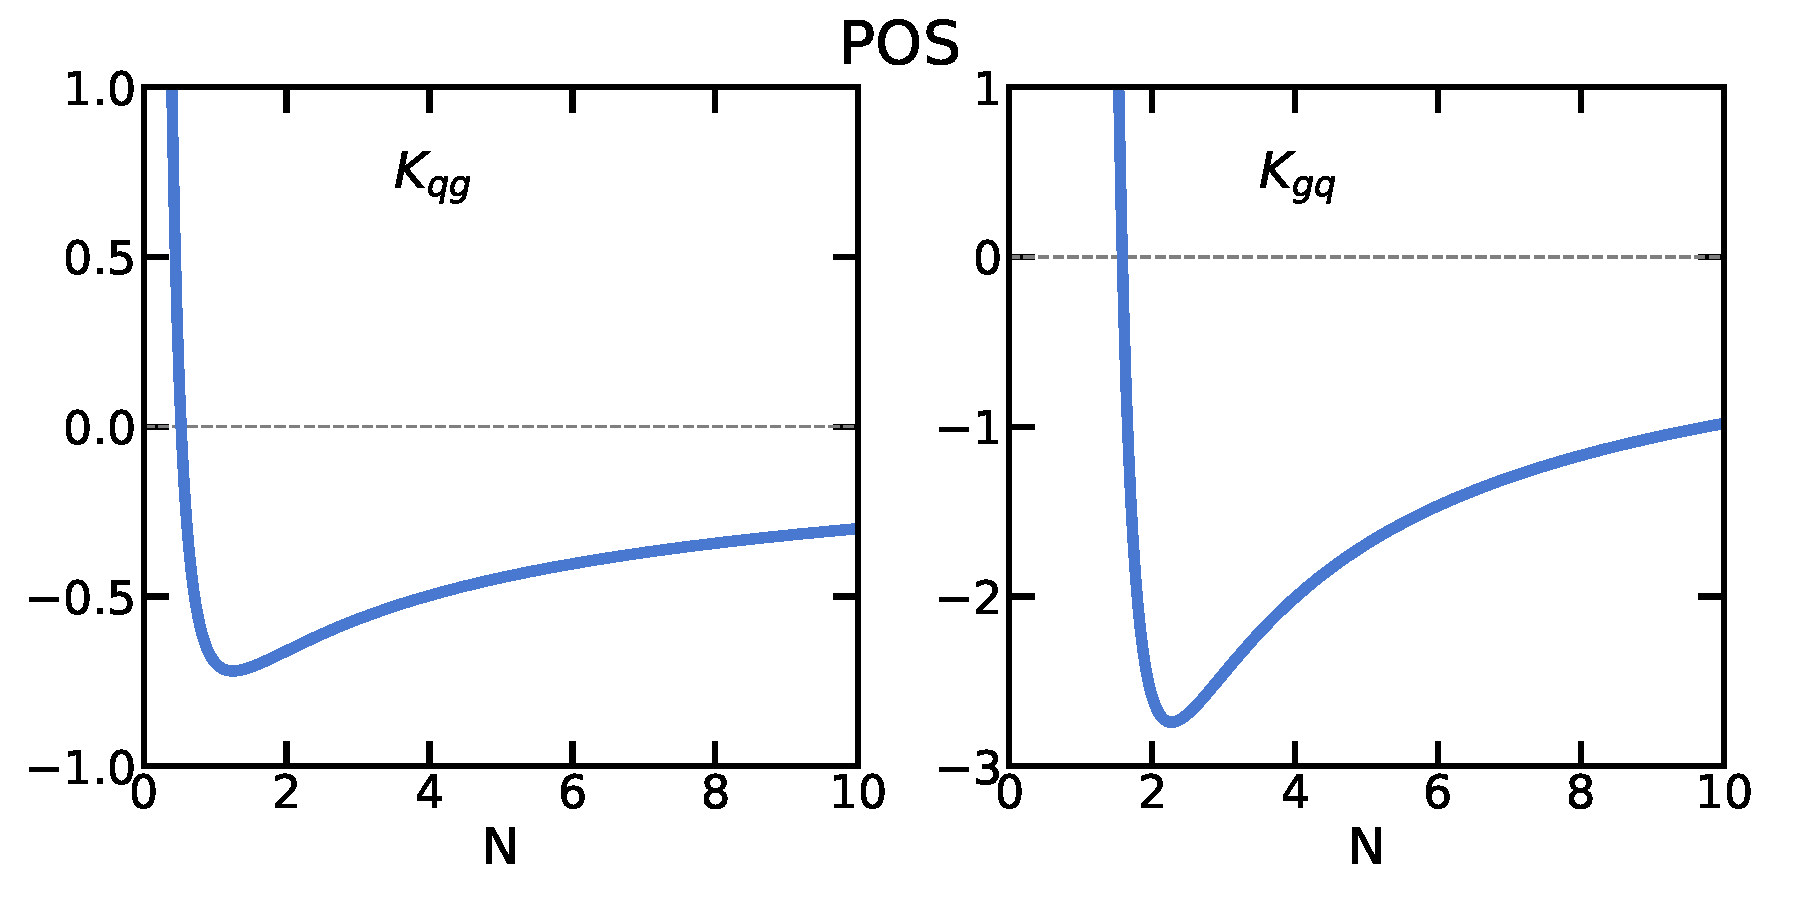
\includegraphics[width=0.85\textwidth]{pictures/kmatrix-offdiagonal-9}
    \end{figure}
\end{frame}

\section{Conclusion}
\begin{frame}{Is it enough?}
    No it's \textbf{not enough}, \textbf{nor needed}.

    \metroset{block=fill}
    \begin{block}{Sufficient}
    It should be noticed that PDF positivity it's still not enough to guarantee
    observables positivity, since the coefficient functions are not bounded to
    be positive in x space in 4 dimensions.
    \end{block}

    \begin{block}{Necessary}
    It's also not necessary, because negative PDF folded with suitable
    coefficient functions can still lead to positive observables.
    \end{block}

    From a practical point of view the positivity of observables is a
    requirement (a \textit{constraint}) that should be still implemented
    separately in a PDF fit.
\end{frame}

\begin{frame}{So why?}
    \vspace*{10pt}
    It is a useful physical constraint on the PDFs, so it will add
    \textbf{more theoretical knowledge} in the fit.

    In practice it cuts out a region of the hypothesis space that should not be
    explore by the fitting algorithm, so

    \begin{center}
        \textit{The main result should be reducing the variance of the fitted PDFs.}
    \end{center}

    \vspace*{25pt}
    \metroset{block=fill}
    \begin{block}{Further scheme optimization}
        It is natural to ask whether the positivity requirement could be more
        restrictive in some factorization schemes than others, but it is
        unclear  whether  and  how  this  question  could  be  answered.
    \end{block}
\end{frame}

\begin{frame}[standout]
    Thanks for your attention
\end{frame}

\appendix

\begin{frame}{Overall structure of the argument}
    \begin{enumerate}
        \item $\msbar$ partonic cross-sections are not positive, we found why
            not a define a factorization scheme that prevent it
        \item enforce momentum sum rules by slightly modifying the former,
            without affecting positivity
        \item considering the scheme change we prove that positivity of PDFs in
            this last scheme prove positivity of PDFs in $\msbar$
    \end{enumerate}
\end{frame}

\begin{frame}{Positive coefficient functions}
    A subtlety is related to the fact that generally partonic cross sections
    are the sum of an ordinary functionof the scaling variable, and a
    distribution localized at the kinematic threshold of the scaling variable.
    Here,by “negative cross section” we mean that the function (i.e.,
    non-distributional part of the cross section) isnegative.  For positivity
    to hold,  the distributional part must also be positive in the sense that
    it gives apositive result when integrated over a positive test function.
    As we shall see below, this condition turns outto be automatically
    satisfied inMS and related schemes
\end{frame}

\begin{frame}{$\pos$ scheme}
POS scheme:
\begin{align*}
 {{C^q{}_q}^{(1)}}^{\pos}(x) &=  {{C^q{}_q}^{(1)}}^{\msbar}(x) \,, \\
 {{C^q{}_g}^{(1)}}^{\pos} (x) &=  {{C^q{}_g}^{(1)}}^{\msbar} (x) - K_{qg}^{\pos} (x) \,,\\
  K_{qg}^{\pos} (x) &=  P_{qg}(x)\left[\log(\frac{(1-x)^2}{x}) - 1\right] \,.
 {{C^g{}_g}^{(1)}}^{\pos}(x)  &=  {{C^g{}_g}^{(1)}}^{\msbar}(x) \,, \\
 {{C^g{}_q}^{(1)}}^{\pos} (x) &=  {{C^q{}_g}^{(1)}}^{\msbar} (x) - K_{gq}^{\pos} (x) \,,\\
  K_{gq}^{\pos} (x) &=  P_{gq}(x)\left[\log(\frac{(1-x)^2}{x})- 1\right]
\end{align*}
Hence, subtraction in the
DPOS scheme amounts to under-subtraction, and if adopted for DIS
coefficient function it leads to a DIS coefficient function
${C^{(1)}_{g}}^{\pos}(x)$ which is actually more positive than that
in the DPOS scheme. This is seen in Fig.~ (right), where
${C^{(1)}_{g}}(x)$ is shown in the $\msbar$, DPOS and POS schemes.
\end{frame}

\begin{frame}{N-space positivity $\neq$ x-space positivity}
    The easy way in \textit{N-space} and Why we need an argument in \textit{x-space}
\end{frame}

\begin{frame}{Non-singlet}
    \begin{description}
        \item[academic] it can be that no positive non-singlet combination
            exists, since it is the subtraction of quarks distributions for two
            different flavors;
        \item[isolated] the same we used the non-singlet to set up the argument
            since the singlet is slightly more complicated, indeed the gluon
            couples to all the flavors in the same way, so any correction
            coming from the gluon-quark mixing in change of scheme is
            annihilated by the non-singlet combination;
    \end{description}
\end{frame}

\begin{frame}{NLL calculation}
    The calculation in $x \to 1$ limit, better not to include in the main body (eq. 50-53)
\end{frame}

\begin{frame}{Momentum Sum Rules}
    Inspection of Eq. immediately shows a possible issue
    with the POS scheme. Indeed, as well known, momentum conservation
    implies the pair of relations between the second Mellin moments of splitting
    functions $\gamma_{qq}(2)+\gamma_{gq}(2)=0$ and
     $2n_f\gamma_{qg}(2)+\gamma_{gg}(2)=0$. This relation is verified in the
    $\msbar$ scheme:  in order for it to remain true  in any scheme obtained
    from $\msbar$, the scheme change matrix must satisfy
    \begin{equation}\label{eq:momcons}
      K_{qq}+K_{gq}=2n_fK_{qg}+K_{gg}\Big|_{N=2}=0 \,,
    \end{equation}
    where by $K_{ij}\Big|_{N=2}$ we denote the second Mellin moment of the
    scheme change matrix elements. This relation is not satisfied by the matrix defined in
    Eqs.

    It might therefore be worth considering a variant of the POS scheme,
    in which momentum conservation is enforced by adding to the diagonal
    elements of the scheme change matrix a contribution which enforces
    momentum conservation. This can be done e.g.\ by adding a soft
    function, which vanishes both as $x\to1$ and $x \to0$. We choose
    \begin{equation}\label{eq:fmom}
      f^{\text{MOM}}(x)= 60 x^2(1-x)^2\,,
    \end{equation}
    which has the property that its second Mellin moment equals one:
    $f^{\text{MOM}}(N=2)=1$. We then define a MPOS scheme as that which is obtained
    from $\msbar$ through a scheme change matrix $K^{\mpos}$ whose
    matrix elements satisfy
    \begin{align}
      \label{eq:mposqq}
      K^{\mpos}_{qq}(x)&= - f^{\text{MOM}}(x) K^{pos}_{gq}\Big|_{N=2} \,,\\
      \label{eq:mposqg}
      K^{\mpos}_{qg}(x)&= K^{pos}_{qg}(x) \,,\\
      \label{eq:mposgq}
      K^{\mpos}_{gq}(x)&= K^{pos}_{gq}(x) \,,\\
      \label{eq:mposgg}
      K^{\mpos}_{gg}(x)&= -2n_f f^{\text{MOM}}(x) K^{pos}_{qg}\Big|_{N=2} \,.
    \end{align}
    The MPOS scheme then automatically satisfies momentum
    conservation. Coefficient functions in the MPOS scheme are shown in
    Figs.~. It is clear that coefficient
    functions, and thus PDFs, remain
    positive in the MPOS scheme: indeed, the off-diagonal coefficient
    functions are unchanged, while the diagonal NLO contributions are
    modified by a small correction which is offset by the large positive
    LO contribution, and in fact in the hadronic case leaves the NLO
    correction positive for all $x$. Hence the MPOS and POS schemes have the same
    positivity properties. We will thus not discuss the MPOS scheme
    any further and restrict the discussion for simplicity to the POS
    scheme.
\end{frame}

\begin{frame}{Heavy quarks}
    Heavy quarks require a separate discussion,  because their factorization
    scheme can bedefined in a variety of ways (see e.g. [19]).  Specifically,
    heavy quarks can be treated in amassive scheme,  in which collinear
    singularities associated to them are regulated by theirmass, so they decouple
    from perturbative evolution. In this scheme no collinear subtraction
    isperformed for massive quarks, so their PDF is given by the unsubtracted Eq.
    (2) and thus itremains a positive (and scale-independent) probability
    distribution to all perturbative orders.Note that nothing prevents this heavy
    quark PDF from having an “intrinsic” component, ofnon-perturbative origin:
    however, in this factorization scheme, the heavy quark PDFs willbe
    scale-independent, and thus positive at all scales.

    However, it is also possible to treat the heavy quark in a massless scheme,
    in which theheavy quark is treated like other massless quarks, namely the
    collinear singularity regulatedby its mass is subtracted according to Eqs.
    (9,20), but withμ2now replaced by the heavyquark mass.  Calculations performed
    in this scheme, with heavy quark mass effects neglected,are accurate for scales
    much larger than the quark mass.  ForQ2m2hthis scheme reducesto the standardMS
    and the previous arguments apply.  However, the massless scheme is inprinciple
    formally defined for all scales, including at the heavy quark mass. This is
    sometimesdone by using the massless scheme for all flavors, but discontinuously
    changing the number offlavors at a matching scale chosen equal to (or of order
    of) the heavy quark mass (zero-massvariable-flavor number scheme,  ZM-VFNS
    [20]).  Below the matching scale the ZM-VFNSscheme  coincides  with  the
    massive  scheme  (with non-evolving  heavy  quark  PDF),  and  atthe matching
    scale the heavy quark PDF changes discontinuously:  the matching condition20 is
    the scheme transformation from the massive to the masslessMS (computed up to
    NNLOin  Ref.  [21]).   At  this  scale,  the  scheme  change  matrix  from  the
    (positive) massive  flavorto massless scheme is a function of the heavy quark
    massmh, rapidly varying with scaleqwhenQ∼mhand unrelated to the scheme change
    fromMS to POS. Hence, the previousarguments do not apply and no conclusions can
    be drawn on on the positivity of the heavy-quark PDF in the massless scheme
    from its positivity in the massive scheme.  Indeed,  forrealistic quark and
    gluons and in the absence of intrinsic component theMS massless-schemecharm PDF
    turns out to be negative for somexvalues when the scale is set equal to
    thecharm mass
\end{frame}

\begin{frame}{Positive to all orders}
    All the discussion so far has been pursued at NLO.  However, the main
    structure of theargument remains true to all perturbative orders.  In
    particular, it is true to all orders thatthe diagonal splitting functions
    are negative at largex:  in fact, at largexto all perturbativeorders they
    behave as1(1−x)+[14].  At higher perturbative orders, coefficient functions
    willcontain higher order powers of ln(1−x), leading to the familiar rise in
    the partonic crosssection  which  is  predicted  to  all  orders  by
    threshold  resummation  [11, 12].   Off-diagonalchannels,  where  negative
    contributions  asx→1  may  and  indeed  are  expected  to  arise,remain
    power  suppressed  in  this  limit.   It  follows  that  the  off-diagonal
    structure  Eq.  (71)of the matrix relating a positive scheme toMS will hold
    true to all orders.  The positivityargument of Sect. 3.2.2 is a direct
    consequence of this structure, and it will thus also holdto all orders.
\end{frame}

\begin{frame}{more motivations}
    \begin{itemize}
        \item pdf should produce positive results also in regions where experimental data are not well known, witho
    \end{itemize}
\end{frame}


\end{document}
